%\documentclass[fleqn]{article}
%\documentclass[twocolumn,10pt]{article} %% original submission
%\documentclass[nocopyrightspace]{sigplanconf}

\documentclass{acm_proc_article-sp}

\usepackage{xspace,amsmath,math-cmds,
            math-envs,inference-rules,times,
            verbatim,alltt,multicol,proof,url}
\usepackage{epsfig}
\usepackage{code} 
%\setlength{\oddsidemargin}{0in}
%\setlength{\evensidemargin}{0in}
%\setlength{\textwidth}{6.5in}
%\setlength{\textheight}{8.5in}

\setlength{\hoffset}{-1in}
\setlength{\voffset}{-1in}

\setlength{\topmargin}{1in}
\setlength{\headheight}{0pt}
\setlength{\headsep}{0pt}

\setlength{\evensidemargin}{.75in}
\setlength{\oddsidemargin}{.75in}

% Text area:

\newdimen{\standardtextwidth}
\setlength{\standardtextwidth}{42pc}

\setlength{\textwidth}{\standardtextwidth}

\setlength{\topskip}{8pt}
\setlength{\columnsep}{1.5pc}
\setlength{\textheight}{54.5pc}


\author{Kenny Q. Zhu \\
	   Shanghai Jiao Tong University\\
       {\small \tt kzhu@cs.sjtu.edu.cn}
	\and Kathleen Fisher \\
	   AT\&T Labs Research\\
       {\small \tt kfisher@research.att.com}
	\and David Walker \\
	   Princeton University\\
       {\small \tt dpw@cs.princeton.edu}}
\date{}
\makeatletter
\let\@copyrightspace\relax
\makeatother

\begin{document}

\newcommand{\cut}[1]{}
\newcommand{\reminder}[1]{{\it #1 }}
\newcommand{\poplversion}[1]{#1}
\newcommand{\trversion}[1]{}

\newcommand{\appref}[1]{Appendix~\ref{#1}}
\newcommand{\secref}[1]{Section~\ref{#1}}
\newcommand{\tblref}[1]{Table~\ref{#1}}
\newcommand{\figref}[1]{Figure~\ref{#1}}
\newcommand{\listingref}[1]{Listing~\ref{#1}}
%\newcommand{\pref}[1]{{page~\pageref{#1}}}

\newcommand{\eg}{{\em e.g.}}
\newcommand{\cf}{{\em cf.}}
\newcommand{\ie}{{\em i.e.}}
\newcommand{\etc}{{\em etc.\/}}
\newcommand{\naive}{na\"{\i}ve}
\newcommand{\role}{r\^{o}le}
\newcommand{\forte}{{fort\'{e}\/}}
\newcommand{\appr}{\~{}}

%\newcommand{\bftt}[1]{{\ttfamily\bfseries{}#1}}
\newcommand{\kw}[1]{\bftt{#1}}
\newcommand{\pads}{\textsc{pads}}
\newcommand{\padsc}{\textsc{pads/c}}
\newcommand{\ipads}{\textsc{ipads}}
\newcommand{\padsl}{\textsc{padsl}}
\newcommand{\blt}{\textsc{blt}}
\newcommand{\ddc}{\textsc{ddc}$^{\alpha}$}
\newcommand{\ddcold}{\textsc{ddc}}
\newcommand{\padsml}{\textsc{pads/ml}}
\newcommand{\padsmlbig}{\textsc{PADS/ML}}
\newcommand{\ddl}{\textsc{ddl}}
\newcommand{\C}{\textsc{c}}
\newcommand{\perl}{\textsc{perl}}
\newcommand{\ml}{\textsc{ml}}
\newcommand{\smlnj}{\textsc{sml/nj}}
\newcommand{\ocaml}{\textsc{o'caml}}
\newcommand{\java}{\textsc{java}}
\newcommand{\xml}{\textsc{xml}}
\newcommand{\xquery}{\textsc{xquery}}
\newcommand{\datascript}{\textsc{datascript}}
\newcommand{\packettypes}{\textsc{packettypes}}
\newcommand{\erlang}{\textsc{Erlang}}

\newcommand{\dibbler}{Sirius}
\newcommand{\ningaui}{Altair}
\newcommand{\darkstar}{Regulus}

%% \newcommand{\IParray}[4]{{\tt Parray} \; #1 \; \[#2, #3, #4\]}

\newcommand{\figHeight}[4]{\begin{figure}[tb]
	\centerline{
	            \epsfig{file=#1,height=#4}}
	\caption{#2}
	\label{#3}
	\end{figure}}


%\twocolumn[\maketitle]

\title{Incremental Learning of System Log Formats}
%\subtitle{[Extended Abstract]}

\author{
\numberofauthors{3}
\alignauthor
  Kenny Q. Zhu \\
  \affaddr{Shanghai Jiao Tong University} \\
  \email{kzhu@cs.sjtu.edu.cn}
\alignauthor
  Kathleen Fisher \\
  \affaddr{AT\&T Labs Research} \\
  \email{kfisher@research.att.com}
\alignauthor
  David Walker \\
  \affaddr{Princeton University} \\
  \email{dpw@cs.princeton.edu}
}

\maketitle

Many applications use the file system as a simple persistent data
store.  This approach is expedient, but it is not robust.  In general,
the overall correctness of such an application dependso on the
collection of files, directories, and symbolic links having some
precise hierarchical organization. Furthermore file system properties
such as file ownership, permissions, and timestamps must have
acceptable values. Unfortunately, current programming languages do not
provide support for documenting assumptions about the file system. In
addition, actually loading data from disk requires writing tedious
boilerplate code.

This paper describes \forest{}, a new domain-specific language for
describing directory structures embedded in \haskell{}. \forest{}
descriptions use a type-based metaphor to specify portions of the file
system in a simple, declarative manner.  \forest{} makes it easy to
connect data on disk to an isomorphic representation in memory
that can be manipulated by programmers as if it were any other
data structure in their program.  \forest{} generates
metadata that describes to what degree the files on disk conform to
the specification, making error detection easy. The system greatly
lowers the divide between on-disk and in-memory representations of
data. \forest{} leverages \haskell{}'s powerful generic programming
infrastructure to make it easy for third-party developers to build
tools that work for any \forest{} description.  We illustrate the use
of this infrastructure to build a number of useful tools, including a
visualizer, permission checker, and description-specific tools for a
number of standard shell tools.

\cut{
We present the design for \forest{} and describe the implementation of
a full working prototype. From a single compact description, the
\forest{} compiler generates a collection of \haskell{} types and
functions for validating and analyzing file system data.  In addition,
\forest{} generates type class instance declarations that make it
possible to exploit powerful generic programming paradigms that allow
third-party developers to build tools for querying, visualizing, and
debugging on-disk data in a generic way. We present examples
illustrating the use of \forest{} on a number of real-world directory
structures and programming tasks, including description-specific
replacements for a number of standard shell tools. Finally, we
formalize the core elements of the language as a simple calculus based
on classical tree logics.}

\category{D.4.9}{Operating Systems}{Systems Programs and Utilities}
\category{D.3.4}{Programming Languages}{Processors}

\terms
Languages, Algorithms

\keywords
Grammar induction, analysis of system logs, domain-specific languages, parsing,
tool generation, ad hoc data, PADS

\section{Introduction}
\label{sec:intro}

\datascript{}~\cite{gpce02}. \packettypes{}~\cite{sigcomm00}. \padsc{}~\cite{fisher+:pads}
and \padsml{}~\cite{mandelbaum+:padsml}. Bro\cite{paxson:bro}. These
are but a few of the many languages designed for describing data
formats. In his classic paper {\em The Next 700 Programming
  Languages}, 1966~\cite{landin:700}, Landin asserts that principled
programming language design involves thinking in terms of ``families
of languages'' and choosing from a ``well-mapped space.''  However,
when it comes to the domain of processing ad hoc data, there is no
well-mapped space and no systematic understanding of the family of
languages one might be dealing with.

In our previous work, we developed the data description calculus
\ddcold{} to capture the core features of many existing data
description languages~\cite{fisher+:next700ddl}, like \padsc{},
\packettypes{} and \datascript{}. Given the broad applicability of
\ddcold{}, we wanted to use it to define the semantics of
\padsml{}. However, the polymorphic types that we wished to include in
\padsml{} can not be formalized with \ddcold{}.  In addition, both
\padsc{} and \padsml{} generate tools from data format descriptions to
{\em print} data in the specified format. For
many applications, printing data correctly can be as important as
parsing it correctly. Yet, our previous work
specified only the type and parsing semantics of \ddcold{}. 

In this work, we address both of these limitations of
\ddcold{}. First, we extend \ddcold{} with abstractions over types to
create \ddc. In the process, we also improve the \ddc\ theory, as
noted in \secref{sec:ddc-sem}. The new \ddc provides basis for
specifying the semantics of \padsml{}. Second, we specify the a
printing semantics for the new \ddc{}.  We used this new
semantics to guide the \padsml{} implementation of printing.
\secref{sec:ddc} presents the extended \ddc{} calculus, focusing on
the semantics of polymorphic types for parsing and the key elements of
the printing semantics.  We show that both parsers and printers in the
\ddc{} are type correct and furthermore that parsers produce pairs of
parsed data and parse descriptors in {\em canonical form}, and that
printers, given data in canonical form, print successfully.

In summary, this work makes the following key contributions:
\begin{itemize}
\item We have defined the formal semantics of both \padsml{} parsers 
and printers. 
\item We have proven our generated code is type safe and
well-behaved as defined by a canonical forms theorem.
\end{itemize}

%%% Local Variables: 
%%% mode: latex
%%% TeX-master: "paper"
%%% End: 


\section{Review of PADS and LearnPADS}\label{sec:review}


\section{Main Algorithm}\label{sec:algo}

To address these problems, we extended \learnpads{} to work
incrementally.  
\figref{fig:overview} illustrates the overall process.
Given a candidate description \cd{D}, the new algorithm uses \cd{D} to parse
the records in the data source.  
It discards records that parse successfully, since these records are
already covered by \cd{D}, but it collects records that fail to parse.
When the algorithm accumulates $M$ such records, where $M$ is a
parameter of the algorithm, it invokes the incremental learning step,
described below, to produce a refined description \cd{D'}.  This refined
description subsumes \cd{D} and describes the $M$
new records.  In addition, the algorithm attempts to preserve as much
of the structure of \cd{D} as possible, so users supplying initial
descriptions can recognize the resulting descriptions. 
The algorithm then takes \cd{D'}
to be the new candidate description and repeats the process until it
has consumed all the input data.
The initial description \cd{D} can either be supplied by a user or it
can be inferred automatically by applying the original algorithm to
$N$ records selected from the data source, where $N$ is another
parameter.  
%Currently, the system selects a mix of $N/3$ consecutive lines
%taken from the beginning, middle, and end of the data source. 


Intuitively, the incremental learning step works by attempting to
parse each of the $M$ records according to the current description
\cd{D}.  It discards the portions of each record that parse correctly.
If a portion fails to parse, that failure will be detected at a
particular node in the description \cd{D}. It collects these failed
portions in an aggregation data structure \cd{A} that mirrors the
structure of \cd{D}.  After thus aggregating all the failures in the $M$
records, the algorithm transforms \cd{D} to accommodate the places where
differences were found (\ie, by introducing options where a piece of
data was missing or unions where a new type of data was discovered).
It then uses the original \learnpads{} algorithm to infer descriptions
for the aggregated portions of bad data. 

In the rest of this section, we present the algorithm in more detail.

\cut{
Intuitively, the incremental learning algorithm takes an initial
description as input, divides the new data into manageable
chunks, and iteratively merges descriptions of these chunks into the
current description.
\figref{fig:overview} illustrates a high level schematic of this
algorithm. A large or streaming data source is input 
to the system in batches. Each batch of data contains $M$ 
records, where $M$ is a parameter of the framework.
%%The state of the system is determined by the current data
%%description which is subject to change as new data streams into the system. 
The initial description
can be supplied by user, or learned from the first batch of the input
data. At each iteration, the system generates a filter program from
the current data description.  This program parses the incoming batch of data
into an aggregted data structure similar to the parse tree of the description.
In this process, the filter program collects ``bad data'' which does not
comform to the current description. The system then invokes the original
\learnpads{} algorithm to learn ``sub-descriptions'' from the bad data, and
merges these sub-descriptions into the current data description to produce
a new description for the next iteration. 
}
\begin{figure}[t]
\centering
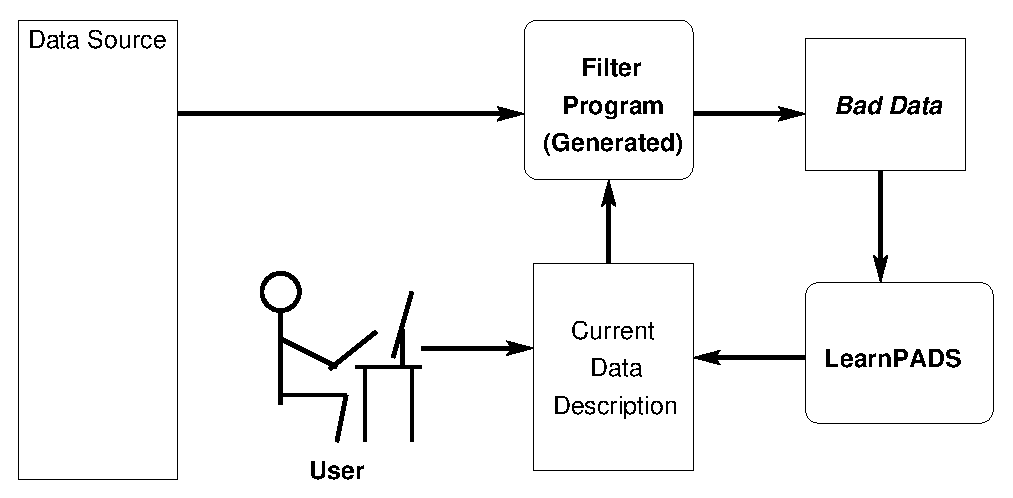
\includegraphics[width=0.9\columnwidth]{overview}
%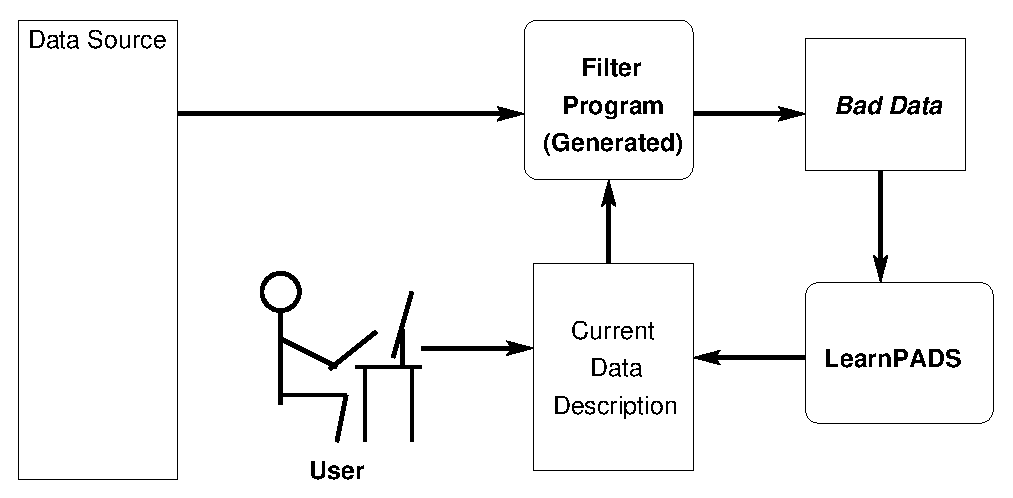
\epsfig{file=overview.eps,width=0.9\columnwidth}
\caption{An Overview of the Incremental Learning Framework}
\label{fig:overview}
\end{figure}

%To address these problems, 
%we extended \learnpads{} to work incrementally.  
%Given a candidate description \cd{D}, the new algorithm uses \cd{D} to parse
%the records in the data source.  
%It discards records that parse successfully, since these records are
%already covered by \cd{D}, but it collects records that fail to parse.
%When the algorithm accumulates $M$ such records, where $M$ is a
%parameter of the algorithm, it invokes the incremental learning step,
%described below, to produce a refined description \cd{D'}.  This refined
%description subsumes \cd{D} and describes the $M$
%new records.  In addition, the algorithm attempts to preserve as much
%of the structure of \cd{D} as possible, so users supplying initial
%descriptions can recognize the resulting descriptions. 
%The algorithm then takes \cd{D'}
%to be the new candidate description and repeats the process until it
%has consumed all the input data.
%The initial description \cd{D} can either be supplied by a user or it
%can be inferred automatically by applying the original algorithm to
%$N$ records selected from the data source, where $N$ is another
%parameter.  
%Currently, the system selects a mix of $N/3$ consecutive lines
%taken from the beginning, middle, and end of the data source. 

\subsection{Preliminaries}

\begin{figure}[t]
{\small 
\begin{code}
\kw{Basic notation}:
c          (a string character)	
s1.s2      (concatenation of strings)
prefix(s)  (set of prefixes of s)
sprefix(s) (set of strict prefixes of s)
\end{code}
\begin{code}
\kw{Descriptions}:
Base ::= Pint | PstringME(re) | PstringFW(e)
\end{code}
\begin{code}
D ::=   
  Base               (Base token)
| Sync s             (Synchronizing token) 
| Pair (x:D1, D2)    (Pair with dependency)
| Union (D1, D2)     (Union)
| Array(D, s, t)     (Array)
| Option D           (Option)
\end{code}
\begin{code}
\kw{Data representation}:
BaseR ::= Str s | Int i | Error
\end{code}
\begin{code}
SyncR ::= Good | Fail | Recovered s 
\end{code}
\begin{code}
R ::=
  BaseR
| SyncR
| PairR (R1, R2)
| Union1R R | Union2R R 
| ArrayR (R list, SyncR list, SyncR)
| OptionR (R option)
\end{code}
\begin{code}
\kw{Aggregation structure}:
A :: = 
  BaseA Base
| SyncA s
| PairA(A1, A2)
| UnionA(Al, Ar)
| ArrayA (A_elem, A_sep, A_term)
| OptionA A
| Opt A
| Learn [s]
\end{code}
}
\caption{Preliminary data structures used in incremental inference}
\label{fig:data-structures}
\end{figure}

\cut{%%%%%%%%%%%%%%%%%%%%%%%%%%%%%%%%%%%%%%%%%
Intuitively, the incremental learning step works by attempting to
parse each of the $M$ records according to the current description
\cd{D}.  It discards the portions of each record that parse correctly.
If a portion fails to parse, that failure will be detected at a
particular node in the description \cd{D}. It collects these failed
portions in an aggregation data structure \cd{A} that mirrors the
structure of \cd{D}.  After thus aggregating all the failures in the $M$
records, the algorithm transforms \cd{D} to accommodate the places where
differences were found (\ie, by introducing options where a piece of
data was missing or unions where a new type of data was discovered).
It then uses the original \learnpads{} algorithm to infer descriptions
for the aggregated portions of bad data. 
}%%%%%%%%%%%%%%%%%%%%%%%%%%%%%%%%%%%%%%%%%%%%%%%%%%%%

\figref{fig:data-structures} defines
the data structures for descriptions \cd{D}, data
representations \cd{R}, and aggregate structures \cd{A}.
In these definitions,  variable \cd{re} ranges over regular expressions,
\cd{e} over host language expressions,
\cd{s} and \cd{t} over strings, and \cd{i} over integers.
%A value with type \cd{D} is the abstract syntax tree of \pads{}
%description: this description is what we want to learn.  
For simplicity of presentation, we assume just three base types: 
integers, strings that match a regular expression and strings with a
fixed width specified by an expression. Synchronizing
tokens, or {\em sync tokens} for short, correspond to string literals
in \pads{} descriptions.  Such tokens, which are often
white spaces or punctuation,
serve as delimiters in the data and are useful for detecting
errors. The binary dependent pairs \cd{Pair (x:D1, D2)} are
a simplicification of PADS more general \kw{Pstruct}s. 
The variable \cd{x} refers to the data parsed by \cd{D1}
and may be used in \cd{D2}. The union \cd{Union (D1, D2)}
provides a choice between descriptions \cd{D1} and \cd{D2}.
An array description
\cd{Array(D, s, t)} has an element type described by \cd{D}, a separator
string \cd{s} that appears between array elements, and a
terminator string \cd{t}. Finally, \cd{Option D} indicates \cd{D} is 
an optional data element.  To resolve ambiguities, unions are
biased towards their first element, arrays are biased towards a longest match
semantics and options are biased towards matching as opposed to not matching.

A term \cd{R} is a parse tree obtained from parsing 
data using a description \cd{D}.  Parsing a base type can result in a
string, an integer or an error.  Parsing a sync token
\cd{Sync s} can give three different results: \cd{Good}, meaning the
parser found \cd{s} at the beginning of the input; \cd{Fail}, meaning
\cd{s} is not a substring of the current input; or \cd{Recovered s'},
meaning \cd{s} is not found at the beginning of the input, but
can be {\em recovered} after ``skipping'' string \cd{s'}.  The parse
of a pair is a pair of representations, and the parse of a union is
either the parse of the first branch or the parse of the second
branch. The parse of an option is either the parse of its body or  empty.
The parse of an array includes a list of parses for the
element type, a list of parses for the separator and a parse for the
terminator which appears at the end of the array.

An aggregation structure accumulates the set of currently
unparseable data fragments whose form must be learned
for inclusion in the grammar.
The aggregation structure mirrors the structure of the description \cd{D} 
with two additional nodes: an \cd{Opt} node and a \cd{Learn} node. 
%Note the difference between {\tt Opt} nodes and {\tt OptionA} nodes. The latter 
%just corresponds to the description {\tt Option D}. 
The \cd{Learn} nodes accumulate extra, unparseable data 
whose structure must be learned.
The \cd{Opt} nodes do the opposite: they denote the fact that
certain data items were missing.  One of the invariants 
of the aggregation structure is that
newly inserted \cd{Opt} nodes always wrap either a \cd{BaseA} or 
a \cd{SyncA} node.

%Once the system infers a description for this accumulated data, it
%splices in the new description in place of the \cd{Learn} node.

\subsection{Incremental Learning Step}
\begin{figure}[t]
\begin{codebox}
incremental_step(D, xs) =
  As = [\kw{init_aggregate}(D)];
  foreach x in xs \{
    Rs = \kw{parse}(D, x);
    As' = [];
    foreach R in Rs \{
      foreach A in As \{
        A' = \kw{aggregate}(A, R); 
        As' = A :: As'
      \}
    \}
    As = As'
  \} 
  best_a = \kw{select_best}(As);
  D' = \kw{update_desc}(D, best_A);  
  return D'
\end{codebox}
\caption{Pseudo-code for the incremental learning step}
\label{fig:inc-learning}
\end{figure}

\figref{fig:inc-learning} gives pseudo-code for the {\em incremental
  learning step}.  The input to this step is the current description
\cd{D} and a batch of data records \cd{xs}.  The \cd{init\_aggregate}
function initializes an empty aggregate according to description
\cd{D}.  During parsing, the algorithm iteratively updates a list of
possible aggregates \cd{As}, seeded with the initial aggregate of
\cd{D}.  For each data record \cd{x}, the algorithm uses the
\cd{parse} function to produce a list \cd{Rs} of possible parses.  It
then calls the \cd{aggregate} function to merge each parse \cd{R} in
the current list of parses with each aggregate \cd{A} in the current
list of aggregates.  (We use `\cd{::}' to denote prepending an element
onto the front of a list.)  When the system finishes parsing all the
input data, the algorithm uses the \cd{select\_best} function to
select the best aggregate from the list of candidate aggregates
\cd{as}.  The \cd{select\_best} function counts the total number of
\cd{Opt} and \cd{Learn} nodes in each of the aggregates, and returns
the one with the smallest number.
The idea is that the aggregate with the smallest number of added nodes is 
more likely to represent a new description
that is the closer to the original description. 
Finally, the \cd{update\_desc} function uses the structure of the best
aggregate to update the previous description \cd{D} to produce the new
current description \cd{D'}.  The \cd{update\_desc} function works by
doing two things.
First, it converts the aggregate structure back to a \pads{} description
with \cd{Opt} nodes translated to \cd{Poption} types. In addition,
it invokes the \learnpads{} format inference
algorithm to learn a sub-description for the data collected 
at each of the \cd{Learn} nodes
and replaces these \cd{Learn} nodes with these new sub-descriptions. 
Second, it uses rewriting
rules to improve the overall structure.
We will discuss these rewriting rules in more
detail in \secref{sec:imp}.

\begin{figure}[t]
%\begin{center}
{\small
\begin{code}
\cdmath\small
\kw{Base}:
(Int (atoi s), m) $\in$ L(Pint,E,s,s')
  if m = (0,0,len(s))
(Error, (1,0,0)) $\in$ L(Pint,E,"",s'), 
  if s $\in$ L((+|-)?[0-9]+) 
  and L([0-9]) $\cap$ prefix(s') = \{\}
(Str s, m) $\in$ L(PstringME(re),E,s,s'),
  if s $\in$ L(re) 
  and m = (0,0,len(s)) 
  and s.s'' $\not\in$ L(re) and s'' $\in$ prefix(s') 
(Error, m) $\in$ L(PstringME(re),E,"",s'), 
  if "" $\not\in$ L(re)
  and m = (1,0,0)
(Str s, m) $\in$ L(PstringFW(e),E,s,s') 
  if E(e) = Int k and s = c1...ck
  and m = (0,0,len(s))
(Error, (1,0,0)) $\in$ L(PstringFW(e),E,"",s') 
  if E(e) $\ne$ Int k for any k
(Error, (1,0,0)) $\in$ L(PstringFW(e),E,"",s') 
  if E(e) = Int k and k > 0
\mbox{}
\kw{Sync}:
(Good, (0,0,len(s))) $\in$ L(Sync(s),E,s,s')
(Recovered s1, m) $\in$ L(Sync(s2),E,s,s')
  if s=s1.s2 and s2 $\not\in$ prefix(s1.s2)
  and m = (1,len(s1),len(s2))
(Fail, (1,0,0)) $\in$ L(Sync(s2),E,"",s')
\mbox{}
\kw{Pair}:
(PairR (R1,R2), (m1 + m2)) 
        $\in$ L(Pair(x:D1, D2),E,s1.s2,s')
  if  (R1, m1) $\in$ L(D1,E,s1,s2.s')
  and (R2, m2) $\in$ L(D2,E[x $\arrow$ R1],s2,s')
\mbox{}
\kw{Main parse function}:
\kw{parse}(D, s) = \{R | (R, m) $\in$ L(D,.,s,"")\} 
\end{code}
%and for all (R',m') $\in$ L(D,.,s,""), m <= m'
}
\caption{Semantics of parsing (selected elements)}
\label{fig:parse-sem}
%\end{center}
\end{figure}

%% \mbox{}
%% \kw{Union}:
%% (Union1R R, m) $\in$ L(Union(D1, D2),E,s,s')
%%   if (R, m) $\in$ L(D1, E, s, s')
%% (Union2R R, m) $\in$ L(Union(D1, D2),E,s,s')
%%   if (R, m) $\in$ L(D2, E, s, s')

%% \kw{Array}:
%%   (ArrayR([R1,...,Rn], [SyncR1,...,SyncR(n-1)], $SyncR_{term}$), m)
%%     $\in$ L(Array(D, $s_{sep}$, $s_{term}$), E, s, s'),
%%         if
%%         s = s1.$s_{sep}$.s2.$s_{sep}$...s(n-1).$s_{sep}$.sn,
%%         lookaheadfori = $s_{sep}$.s(i+1).....sn.s'
%%         lookaheadforsepi = s(i+1)....sn.s'
%%         s' = s1'.lookaheadforterm

%%         forall i $\in$ [1, n]:
%%           (Ri, mi) $\in$ L(D, E, si, lookaheadfori),
%%         forall i $\in$ [1, n-1]:
%%           (SyncRi, m(s,i)) $\in$ L(Sync($s_{sep}$), E, $s_{(sep,i)}$, lookaheadforsepi),

%%         ($SyncR_{term}$, $m_{term}$) $\in$ L(Sync($s_{term}$), E, s1', lookaheadforterm),
%%         m = $\sum_{i= 1}^{n} mi$ + $\sum_{i=1}^{n-1} m(s,i)$ + $m_{term}$
%% \mbox{}
%% \kw{Option}:
%% (OptionR (SOME R), m) $\in$ L(Option D, E, s, s')
%%   if (R, m) $\in$ L(D, E, s, s')
%% (OptionR (NONE), m) $\in$ L(Option D, E, "", s')
%%   if (R, m) $\in$ L(D, E, "", s')



\subsection{Parsing}
\label{sec:parse}
Our parser is a top-down recursive descent parser
that performs error detection and recovery using synchronizing tokens.
\figref{fig:parse-sem} describes the most important elements
of the parsing algorithm.  For simplicity and brevity,
the algorithm is described abstractly
using a relation with the form 
$(R, m) \in L(D, E, s, s')$.  This relation may be
read as affirming that ``within an environment $E$, a description $D$
can be parsed, generating parse tree $R$ with correctness metric $m$, 
while consuming string $s$, and stopping prior to consuming lookhead 
string $s'$''.  The environment $E$ is a mapping from variable names
$x$ to parse trees $R$.  This environment is used to record the
binding of variables to parse trees introduced by PADS dependent
pair construct.
The {\em parse metric} $m$ measures the quality of a parse. It is a 
triple: ($e$, $s$, $c$), where the $e$ is the number of tokens
with parse errors, $s$ is the number of 
characters skipped during \cd{Sync} token recovery, 
and $c$ is the number of characters correctly parsed. 
To sum two parse metrics, we sum their components:
$(e1, s1, c1) + (e2, s2, c2) = (e1 + e2, s1 + s2, c1 + c2)$.
We compare parse metrics by comparing the ratios of correctly
parsed characters against erroneous tokens and skipped characters:
\[
(e1, s1, c1) \ge (  e2, s2, c2)~ \rm{iff}~ \frac{c_1}{s_1+c_1} \ge \frac{c_2}{s_2 + c_2}
\]

\subsection{Aggregation}
\begin{figure}[t]
\centering
\begin{code}
\cdmath
\kw{Opt}:
  Opt a + Error $\goto$ Opt a
  Opt a + b     $\goto$ Opt b::a
\mbox{}
\kw{a : [Base]}:
  a + Error $\goto$ Opt a
  a + b     $\goto$ b::a
\mbox{}
\kw{a : [Sync s]}: 
  a + Good $\goto$ Good :: a
  a + Fail $\goto$ Opt a
  a + Recovered s' $\goto$ (Opt(l [s'], Good :: a)
\mbox{}
\kw{Opt a : Opt [Sync s]}: 
  Opt a + Good $\goto$ Opt (Good :: a)
  Opt a + Fail $\goto$ Opt a
  Opt a + Recovered s' $\goto$ 
    (Opt (l [s]), Opt (Good :: a))
\mbox{}
\kw{(Opt(l Ss), a) : Opt L * [Sync s]}:
  (Opt(l Ss), a) + Good $\goto$ 
    (Opt(l Ss), Good :: a)
  (Opt(l Ss), Opt a) + Fail $\goto$ 
    (Opt(l Ss), Opt a)
  (Opt(l Ss), Opt a) + Recovered s' $\goto$ 
    (Opt(l s':: Ss), Opt Good :: a)
\mbox{}
\kw{Pair(x:D1, D2)}:
  PairA($a_1$, $a_2$) + PairR($r_1$, $r_2$) $\goto$ 
    PairA($a_1\prime$, $a_2\prime$),
    if  $a_1 + r_1 \goto a_1\prime$
    and $a_2 + r_2 \goto a_2\prime$
\end{code}
\caption{Semantics of aggregation (selected elements)}
\label{fig:aggr-sem}
\end{figure}

%% \kw{Opt a : Opt [Base]}:
%%   Opt a + Error $\goto$ Opt a
%%   Opt a + b     $\goto$ Opt b::a
%% \mbox{}
%% \kw{a : [Base]}:
%%   a + Error $\goto$ Opt a
%%   a + b     $\goto$ b::a
%% \mbox{}
%% \kw{a : [Sync s]}: 
%%   a + Good $\goto$ Good :: a
%%   a + Fail $\goto$ Opt a
%%   a + Recovered s' $\goto$ (Opt(l [s'], Good :: a)
%% \mbox{}
%% \kw{Opt a : Opt [Sync s]}: 
%%   Opt a + Good $\goto$ Opt (Good :: a)
%%   Opt a + Fail $\goto$ Opt a
%%   Opt a + Recovered s' $\goto$ 
%%     (Opt (l [s]), Opt (Good :: a))
%% \mbox{}
%% \kw{(Opt(l Ss), a) : Opt L * [Sync s]}:
%%   (Opt(l Ss), a) + Good $\goto$ 
%%     (Opt(l Ss), Good :: a)
%%   (Opt(l Ss), Opt a) + Fail $\goto$ 
%%     (Opt(l Ss), Opt a)
%%   (Opt(l Ss), Opt a) + Recovered s' $\goto$ 
%%     (Opt(l s':: Ss), Opt Good :: a)
%% \mbox{}
%% \kw{Pair(x:D1, D2)}:
%%   PairA($a_1$, $a_2$) + PairR($r_1$, $r_2$) $\goto$ 
%%     PairA($a_1\prime$, $a_2\prime$),
%%     if  $a_1 + r_1 \goto a_1\prime$
%%     and $a_2 + r_2 \goto a_2\prime$

%% \mbox{}
%% \kw{Union(D1, D2)}:
%%   UnionA($a_l$, $a_r$) + Union1R $r_l \goto$ 
%%     UnionA($a_l\prime$, $a_r$)
%%     if $a_l + r_l \goto a_l\prime$
%%   UnionA($a_l$, $a_r$) + Union2R $r_r \goto$ 
%%     UnionA($a_l$, $a_r\prime$)
%%     if $a_r + r_r \goto a_r\prime$

%% \kw{Array(D, $D_{sep}$, $D_{term}$)}:
%%   ArrayA($a_e, a_s, a_t$) + ArrayR(elems, seps, term) $\goto$ array($a_e\prime, a_s\prime, a_t\prime$)
%%   if 
%% 	$a_e$ ++ elems $\goto a_e\prime$
%% 	$a_s$ ++ seps  $\goto a_s\prime$
%% 	$a_t$ +  term  $\goto a_t\prime$

%% \kw{Option D}:
%%   OptionA a + OptionR (SOME r) $\goto$ OptionA a' if a + r $\goto$ a'
%%   OptionA a + OptionR (NONE) $\goto$ OptionA a 

%% \kw{Aggregation of list}:
%%   a ++ [] $\goto$ a

%%   a ++ (r :: rs) $\goto$ a'' 
%%   if 
%% 	a + r $\goto$ a'
%% 	a ++ rs $\goto$ a''

Aggregation is the process of merging a parse tree, which may contain
errors, into an aggregation structure.  Aggregation is relatively
straightforward and intuitive. 
\figref{fig:aggr-sem} defines how we do aggregation
for several of the important cases by defining a function
$A + R \goto A'$ where $A$ is the initial aggregate data structure,
$R$ is the parse tree and $A'$ is the new aggregate.

\subsection{Examples}
To illustrate the parsing and aggregation phases of the algorithm, we
introduce a simple example.
Suppose we have a description $d$, comprised of a pair of an integer and a sync token ``\cd{*}'',
and we are given the following three lines of new input:

{\small \texttt{
\begin{tabular}{l}
5*\\
abc*\\
8\$\\[1ex]
\end{tabular}}
}

\noindent
\figref{fig:parse} shows the three data representations that result
from parsing the lines, which we call $r_1$, $r_2$ and $r_3$,
respectively. Notice the first line parsed without errors, the second
line contains an error for \cd{Pint} and some unparsable data ``{\tt
  abc}'', and the third contains a \cd{Fail} node because the
sync token \cd{*} was missing.  \figref{fig:aggregate} shows the aggregation
of $r_1$ to $r_3$ starting from an empty aggregate. In
general, \cd{Error} and \cd{Fail} nodes in the data representation
trigger the creation of \cd{Opt} nodes in the aggregate, while
unparsable data is collected in \cd{Learn} nodes.

\begin{figure}[t]
\begin{center}
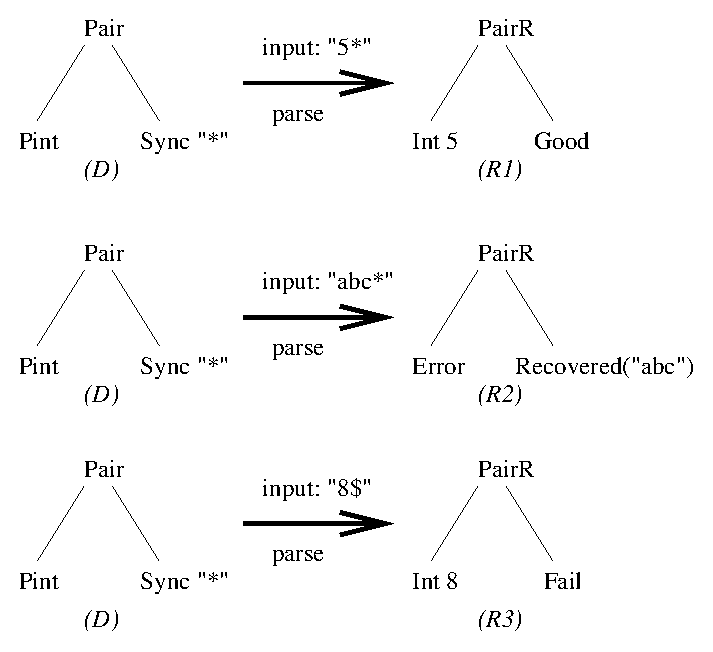
\includegraphics[width=0.8\columnwidth]{parse}
%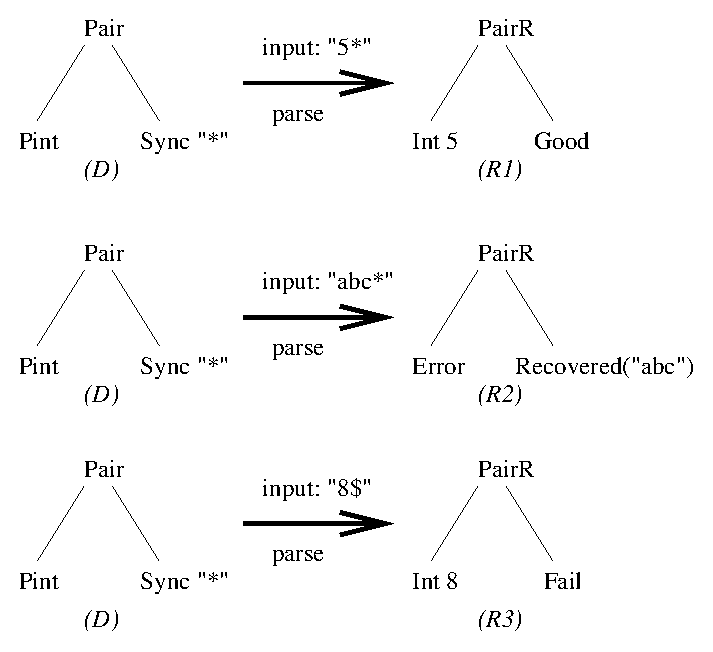
\epsfig{file=parse.eps, width=0.8\columnwidth}
\caption{Result of parsing three input lines}\label{fig:parse}
\end{center}
\end{figure}

\begin{figure*}[t]
\begin{center}
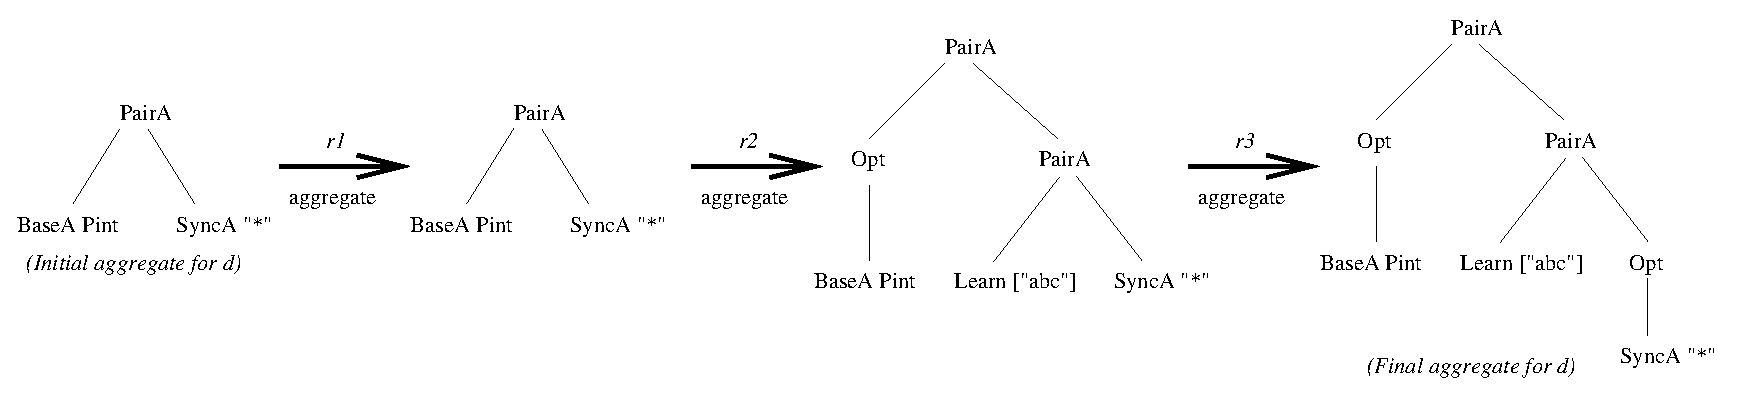
\includegraphics[width=2\columnwidth]{aggregate}
%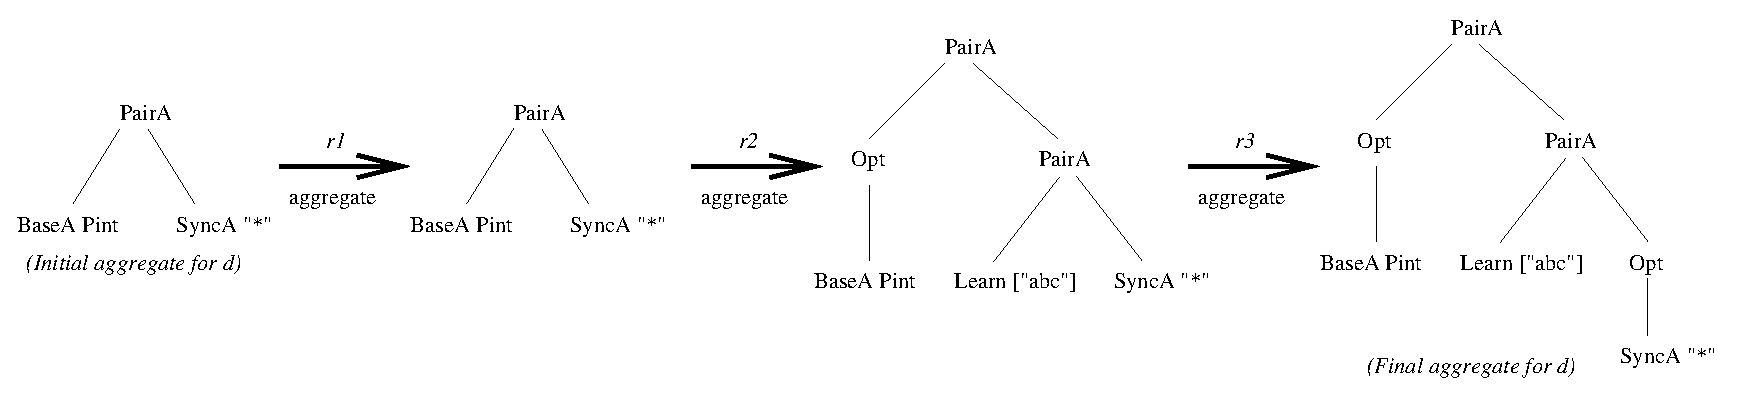
\epsfig{file=aggregate.eps, width=2\columnwidth}
\caption{Aggregation of three parses}\label{fig:aggregate}
\end{center}
\end{figure*}


%\begin{codebox}
%parse_all (d, x) =
%  switch (d) \{
%    case Pint =>  
%      (s, remainder) := match_prefix(x, "[0-9+\-]+");
%      if s != "" then return (Int s, remainder)
%      else return [(Error, x)];
%    case PstringME(re) => 
%      (s, remainder) := match_prefix(x, re);
%      if s != "" then return (Str s, remainder)
%      else return [(Error, x)];
%    case Sync s => 
%      (s', prefix, remainder) := match(x, s);
%      if s' = s and prefix = "" then return (Good, remainder)
%      elseif s' = "" then return (Fail, remainder)
%      else return [(Recovered prefix, remainder)]
%    case (x:d1, d2) =>
%      rs1 := parse_all (d1, x);
%      rs2 := [];
%      foreach (r1, remainder) in rs1 \{
%        (r2, remainder2) := parse_all (d2, remainder);
%        rs2 := rs2 + [((r1, r2), remainder2)]
%      \}
%    case (d1 + d2) => 
%	parse_all(d1, x) @ parse_all(d2, x)
%    case d array(sep, term) =>
%  \} 
%\end{codebox}    
%

\cut{%%%%%%%%%%%%%%%%%%%%%%%%%%%%%%%%

The {\tt parse\_all} function takes a description $d$ and an input string $x$, and returns
a list of all possible parses along with their respective ending position in the input. 
This function implements a standard recursive descent parser which recursively matches the
description structure (and sub-structures) with the input. To parse a pair $x: d_1 * d_2$, 
we first call {\tt parse\_all} on $d_1$ and get a list of parses. 
And then for each of the parse $r_1$ and corresponding end position, we bind $x$ to $r_1$ in
a private environment and  parse $d_2$ to get parses $l_2$. 
Finally for each parse $r_2$ in $l_2$ and each parse $r_1$ in $l_1$, 
construct a representation $(r_1, r_2)$, and return a list of all such pairs.
To parse a union $d_1 + d_2$, we simply return the concatenation of list of parses from
parsing $d_1$ and the list of parses from parsing $d_2$. To parse $d~ array(s, t)$,
we repeatedly attempt to parse $d$ until there's no more progress in the input.
And in each iteration, we also add parses generated from parsing $t$ as well, as if
the array has been terminated at this iteration. Figure \ref{fig:parse_base}
shows the {\tt parse\_base} function which parses a base token. The {\tt match\_prefix}
function matches the prefix of an input string with a regular expression and returns
the matched string and the remainder in the input. The {\tt match} function looks for
the first match of $s$ in input $x$, and returns the matched string $s'$, the prefix string
in $x$ before $s'$, and the remainder in the input.

\begin{figure}[t]
\begin{codebox}
parse_base (b, x) =
  switch (b) \{
  case Pint => 
    (s, suffix) := match_prefix(x, "[0-0+\-]+");
    if s <> "" then return [(Int s, suffix)];
    else return [(Error, x)]
  case PstringME(re) => 
    (s, suffix) := match_prefix(x, re);
    if s <> "" then return [(Str s, suffix)];
    else return [(Error, x)];
  case Sync s => 
    (s', prefix, remainder) := match(x, s);
    if s' = s and prefix = "" then 
      return (Good, remainder)
    elseif s' = "" then 
      return (Fail, remainder)
    else return [(Recovered prefix, remainder)]
  \}
\end{codebox}
\caption{Function to parse a base token or a sync token} \label{fig:parse_base}
\end{figure}

As an example, let $d$ be {\tt (Pint, Sync "|") + (PstringME "[a-z]+", Sync "|")}, 
and $x$ be ``\verb#abc|#''. {\tt parse\_all(d, x)} gives the following two possible parses:
{\small
\begin{verbatim}
  inl (Error, Recovered "abc")
  inr (Str "abc", Good)
\end{verbatim}
}

The {\tt aggregate} function adds a parse into an existing aggregate structure. When there is
no errors in the parse, it makes no changes to the aggregate. If the parse contains 
an error or failure for parsing token $b$, then the aggregate component 
$b$ is transformed to $opt~ b$, to indicate that $b$ node is optional. 
If a parse contains a recovered data $Recovered~ r$, then
a optional learn node will be created before the sync node. And the new aggregate component will be
$(opt (l [r]),~ Sync~ s)$. If the aggregate structure already contains the learn node before this
sync node, then recovered data $r$ will be added to the list under $l$.


}%%%%%%%%%%%%%%%%%%%%%%%%%%%%%%%%% END OF CUT %%%%%%%%%%%%%%%%

% - problem definition (as close to the previous description as possible) (but we don't
%   have a metric to measure how close yet, do we want to mention tree edit distance??)
% - overview of algorithm: parsing + aggregating + rewriting
% - parsing algo (parse rep, score metric, pseudo-code)
% - aggregating algo (in pseudo code)
% - selection of top aggregates
% - update original description
% - rewriting rules (data independent, data dependent, OptsTable)




\section{Implementation}\label{sec:imp}

For purposes of presentation, we have described an idealized and
unoptimized algorithm.  Our actual implementation includes a number of
refinements to improve the quality of the description and/or reduce the
inference time.  In this section, we discuss some of these refinements.

\subsection{Token families}
So far, parsing a \cd{Sync} token yields
one of three results: \cd{Good}, \cd{Fail} or \cd{Recovered}. 
In the actual implementation, a \cd{Sync} token can be not only a constant string, but also
a constant integer, an integer range or a combination thereof.
Consider parsing the token \cd{Sync (Str "GET")} when
the current input starts with ``POST.'' The
\cd{parse\_base} function indicates the result should be \cd{Fail}.
In reality, the input ``POST'' is in the same {\em family} as ``GET,'' 
\ie{}, a word,
and it may very well be that this \cd{Sync} token should have been 
an enumeration of words rather than a single word.
To handle such cases, we created a fourth type of parse node, \cd{Partial}, 
to indicate that the input belongs to the same family as the expected
token but does not match exactly, \ie, it is {\em partially} correct.
During aggregation, partial nodes cause the description 
to be specialized to include the additional values.  In the above example, the aggregate 
function will change the description to \cd{Sync (Enum [Word "GET", Word "POST"])}.
Such partial nodes reduce the number of parsing errors
and produce more compact and meaningful descriptions.


\subsection{Rewriting rules}
When the incremental learning algorithm produces a refined description
from an aggregate, the algorithm applies rewriting rules
to the new description to improve its quality and readability.
Most of the rules are data-independent and inherited from \learnpads{}, such as 
removing degenerate lists and flattening nested structs and unions.
We introduce one new {\em data dependent} rule called {\em MergeOpts}
to optimize a type pattern that occurs frequently during incremental
learning.  Recall that the aggregate function
introduces \cd{Opt} nodes above a \cd{BaseA} or \cd{SyncA} node 
whenever the corresponding \cd{Base} or \cd{Sync} token in the description failed to 
parse. When faced with an entirely new form of data, 
the algorithm is likely to introduce a series of \cd{Opt} nodes as
each type in the original description fails in succession. 
The {\em MergeOpts} rule collapses these consecutive \cd{Opt} nodes if they
are correlated, \ie{}, either they are all always present or all always
absent.  To verify this correlation, the algorithm maintains a
table that records the branching decisions when parsing each
data line. It uses this table to determine whether to merge
adjacent \cd{Opt} nodes during rewriting. 
\figref{fig:opts} illustrates the effect of this rule.  In the figure,
$S$ denotes a struct and $B$ a base token.

\begin{figure}[t]
\begin{center}
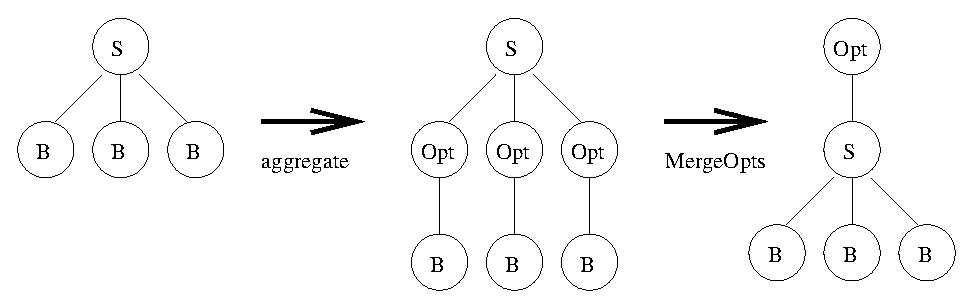
\epsfig{file=opts.eps,width=\columnwidth}
\caption{MergeOpts rewriting rule}\label{fig:opts}
\end{center}
\vskip -2ex
\end{figure}


\subsection{Performance}
The pseudo-code in \figref{fig:inc-learning} suggests the number of
aggregates is of the order $O(m ^ n)$, where $m$ is the maximum number of
parses for a line of input  and $n$ is the number of lines to
aggregate.  Clearly, this algorithm will not scale 
unless $m$ and $n$ are bounded.

We have implemented several optimizations to limit the number of 
parses and aggregates. First, we do not return all possible
parses when parsing a description component \cd{D}. 
Instead, we rank the parses by a metric that
measures their quality and return only the top $k$. The metric is
a triple: 
$m = (e,~ s,~ c)$,
where $e$ is the number of errors, $s$ is the number of 
characters skipped during \cd{Sync} token recovery, and $c$ is the number
of characters correctly parsed. The metric is considered \textit{perfect} if $e = 0$.
Metric $m_1$ is better than $m_2$ if $m_1$ is perfect and $m_2$ is not, or
if 
\[\frac{c_1}{s_1+c_1} > \frac{c_2}{s_2 + c_2}.\]

In practice, \cd{parse} returns a list of
{\em parse triples} $(r,~m,~j)$, where $r$ is the data representation of
the parse, $m$ is the metric associated with $r$, and
$j$ is the position in the input after the parse.
We define a \cd{clean} function that first partitions the
triples into groups that share the same 
{\em span}, \ie{}, the substring of the input consumed by the parse.
For each group, \cd{clean} retains all perfect parses. If 
none exists, it retains the best parse in the group. 
We justify discarding the other triples because
given a description $d$ and a fixed span, we always
prefer the parse with the best metric. This idea is
similar to the dynamic programming techniques used in 
Earley Parsers \cite{earley-parser}. Finally \cd{clean} returns all
the perfect triples plus up to the top $k$ non-perfect triples.
The \cd{clean} function reduces the number of bad parses 
to a constant $k$ while guaranteeing that if there is a
perfect parse, it will be returned. 

A second optimization, which we call {\em parse cut-off}, terminates a
candidate parse when parsing a struct with multiple
fields $f_1$, $f_2$, ..., $f_n$ if the algorithm encounters 
a threshold number of errors in succession. 
This technique may result in no possible parses for the
top-level description.  In this case, we restart the process
with the parse cut-off optimization turned off. 
A third optimization is memoization.
The program keeps a global memo table indexed by the pair of a
description \cd{D} and the beginning position for parsing \cd{D} which
stores the result for parsing \cd{D} at the specific position.
Finally, we bound the total number of aggregates the
algorithm can produce by selecting the top
$k$ aggregates with the fewest number of \cd{Opt} and \cd{Learn}
nodes. 



%\subsection{Objectives}
%
%The purpose of the experiment is to show the following points:
%\begin{itemize}
%\item the learning engine produces *accurate* and *concise* descriptions compared to a human
%expert's descriptions but costs just a fraction of the time; 
%\item it handles a variety of data formats; 
%\item the refinement step significantly improves the structure; 
%\item it is able to produce a description that is sufficiently accurate with 
%much smaller training sets (overfitting vs. underfitting); 
%\item demonstrate that there exists a correlation between sample size, execution time and accuracy,
%and the min sample size required to achieve certain accuracy correlates with the 
%data complexity.
%\end{itemize}

We conducted a series of experiments to study the learning algorithm
and measure its performance. In this section, we will show that
\begin{itemize}
\item the learning engine is capable of handing a variety of data formats;
\item while the initial structure discovery generates a reasonably
good candidate, the refinemnt phase siginificantly improves the
quality of the description through rewritings; 
\item the final output of the learning system is highly competitive
when compared with descriptions written by a human expert 
in terms of accuracy and conciseness; 
\item it is possible to learn from a small training set and produce
a relatively accurate description at a fraction of the cost;
\item there exists a positive correlation between the structural complexity
of the data and the minimum training size required to achieve certain
accuracy.
\end{itemize}

\subsection{Preliminaries}
\begin{table*}
\begin{center}
\begin{tabular}{|l|c|c|c|c|c|c|c|l|} \hline
Data source	& Chunks & Bytes	& Mode  &Header	& Array	& Group & Msgs 	& Comments \\ \hline \hline
1967Transactions.short	& 999	& 70929	& line	& no	& no	& no	& no	& transaction records \\ \hline
MER\_T01\_01.cvs	& 491	& 21731 & line  & yes	& no	& yes	& no	& comma-separated records\\ \hline
ai.3000		& 3000		& 293460 & line	& no	& no	& yes	& no	& web log of Amnesty International \\ \hline
asl.log &	1500	& 279600	& line	& no	& no	& yes	& no	& log file of Mac ASL \\ \hline	
boot.log	& 262	& 16241		& line	& no	& no	& no	& yes	& Mac OS boot log \\ \hline
crashreporter.log & 441	& 50152 	& line	& no	& no	& no	& yes	& original crashreporter daemon log \\ \hline
crashreporter.mod & 441	& 49255		& line	& no	& no	& no	& yes	& modified crashreporter daemon log \\ \hline
dibbler.1000	& 999	& 142607 	& line	& yes	& yes	& no	& no	& AT\&T phone provision data \\ \hline
ls-l.txt	& 35	& 1979		& line	& yes	& no	& no	& no	& Stdout from Unix command ls -l \\ \hline
netstat-an	& 202	& 14355		& block	& yes	& no	& no	& no	& output from netstat -an \\ \hline
page\_log	& 354	& 28170		& line	& no	& no	& no	& no	& printer logs \\ \hline
quarterlypersonalincome & 62	& 10177	& line	& yes	& no	& yes	& no	& spread sheet \\ \hline
railroad.txt	& 67	& 6218		& line	& yes	& yes	& yes	& no	& US rail road info \\ \hline
scrollkeeper.log & 671	& 66288		& line	& no	& no	& no	& yes	& log from cataloging system \\ \hline
windowserver\_last.log & 680	& 52394	& line	& no	& no	& no	& yes	& log from LoginWindow server on Mac \\ \hline
yum.txt		& 328	& 18221		& line	& no	& no	& no	& no	& log from package installer Yum \\ \hline
\end{tabular}
\caption{Benchmark profile} \label{tab:benchmarks}
\end{center}
\end{table*}

The original data sources we used in the experiments are listed in Table \ref{tab:benchmarks}.
These range from personal spread sheet, to government records to system logs, and 
represent vastly different formats. Some benchmarks are large with a few thousand
chunks or records, while others are small with just a few dozen lines. As we will see later
that the size of the data source has some implications in the training performance.
Most of the data files are line based, which means a line represent a data record, with
the exception of netstat-an in which data come in blocks or multiple lines.
Many of the formats include headers or footers which may complicate the descriptions.
From a human point of view, dibbler.1000 and railroad.txt consist of some special
character separated arrays. The ``Group'' column in the table shows if a data source
contain groupings delimited by special characters such as [, ], or quotations.
The ``Msgs'' column indicates whether the data source contains complex English text.
We include two versions of crashreporter.log: an original file ``crashreporter.log''
and ``crashreporter.log.mod'' with some of the date information replaced by ``-''. 
The latter has been used as an example in Section \ref{sec:review}. 

The system that executed the experiments is an 
Apple PowerBook G4 with a 1.67 GHz Processor and 512 MB DDR RAM 
running on Mac OS X 10.4 Tiger. 

\begin{table}
\begin{center}
\begin{tabular}{|l|c|c|c|} \hline
		&  Time to prod.	& MDL score 	& Parsing accuracy 	\\ \hline
HW IR	& -			& X		& -			\\ \hline	
HW PADS	& X			& -		& X			\\ \hline	
INF IR 	& -			& X		& -			\\ \hline
INF PADS & X			& -		& X			\\ \hline 
\end{tabular}
\caption{Measurement for the representations} \label{tab:metrics}
\end{center}
\end{table}

For any of the given data sources, there exists four different representations in 
our experiments: hand-rewritten PADS by human expert (HW PADS), hand-rewritten IR directly
translated from the HW PADS (HW IR), inferred IR from the learning engine (INF IR), and
inferred PADS description which is automatically translated from the INF IR (INF PADS). 
Note that as IR has a simplified language and is not as powerful as the full-fledged
PADS, the HW PADS does not use those features not available in IR and hence it is
not fully optimized. 
Nonetheless, the HW PADS and HW IR are thought to be ``pretty good'' descriptions of
the data and are used as control in the comparisons below. 
In general, we measure the time to produce the descriptions, the MDL scores of
and the parsing accuracy of the descriptions. 
Table \ref{tab:metrics} shows what we measure for each of the four representations.

\subsection{Experiments}
\begin{table*}
\begin{center}
\begin{tabular}{|l||r|r|r|r||r|r|c|} \hline
Formats 	 & Inf time (s) 	& Ref time (s) 	& Total time (s) & HW time (h) & Inf score 	&Ref score	& HW score \\ \hline \hline
1967Transactions.short & 0.20&      2.32&      2.56 	& 4.0 & 0.295 	&0.218 		&0.268		 \\ \hline
MER\_T01\_01.csv & 0.11&      2.80&      2.92 	& 0.5 & 0.648 	&0.112		&0.138		 \\ \hline
ai.3000          & 1.97&      26.35&     28.64	& 1.0 & 0.503	&0.332		&0.338		 \\ \hline
asl.log          & 2.90&      52.07&     55.26	& 1.0 & 0.630	&0.267		&0.361		 \\ \hline
boot.log         & 0.11&      2.40&      2.53 	& 1.0 & 0.620	&0.481		&0.703		 \\ \hline
crashreport.log   & 0.12&      3.58&      3.73 	& 2.0 & 0.607	&0.328		&0.348		 \\ \hline
crashreport.log.mod & 0.15&      3.83&      4.00 	& 2.0 & 0.612	&0.329		&0.347		 \\ \hline
dibbler.1000     & 2.24&      5.69&      8.00 	& 1.5 & 0.602	&0.470		&0.438		 \\ \hline
ls-l.txt         & 0.01&      0.10&      0.11 	& 1.0 & 0.559	&0.333		&0.401		 \\ \hline
netstat-an       & 0.07&      0.74&      0.82 	& 1.0 & 0.413	&0.394		&0.319		 \\ \hline
page\_log        & 0.08&      0.55&      0.65 	& 0.5 & 0.540	&0.107		&0.353		  \\ \hline
quarterlypersonalincome & 0.07&      5.11&      5.18 	& 48  & 0.544	&0.367		&0.354		\\ \hline
railroad.txt     & 0.06&      2.69&      2.76 	& 2.0 & 0.715	&0.506		&0.522		 \\ \hline
scrollkeeper.log & 0.13&      3.24&      3.40 	& 1.0 & 0.625	&0.354		&0.352		 \\ \hline
windowserver\_last.log  & 0.37&      9.65&      10.07	& 1.5 &0.618		&0.241		&0.267		 \\ \hline
yum.txt          & 0.11&      1.91&      2.03 	& 5.0 &0.827		&0.305		&0.474		 \\ \hline
\end{tabular}
\caption{Main results (Inf: structure inference, Ref: Refinement, HW: Hand-written)}
\label{tab:results}
\end{center}
\end{table*}

We first hand-coded all 16 formats in PADS and IR and measure timings and the scores 
of supposedly good descriptions (see HW time column in Table \ref{tab:results}). 
Several formats takes a few hours and up to 2 days(!) to complete because these were the very first 
PADS descriptions ever written by this person. It is obvious that coding description
in PADS is a daunting task for a novice despite that he is a computer science PhD!
To score a given HW IR, we wrote a simple recursive-descent parser with backtracking
for our IR so that the original data can be populated into the IR structure for
correct scoring of the data complexity which is the second component of the MDL score.
After a few attempts and modifications, the HW PADS descritions parses all 
the original data files with 100\% accuracy.

Next we ran the learning system on all 16 data files in their entirety, 
measured timings for structure inference, refinement and the total time which includes
printing out the PADS descriptions and other overhead. 
For accurate timing measurements, run each data format 10 times, and take the average 
after removing the best and the worst times.
We also recorded the scores of both the initial structure and the final structure after refinement.
All these measurements are included in Table \ref{tab:results} as well.
The generated PADS descriptions parses all original data files with 100\% accuracy,
therefore the correctness of the learned formats is guaranteed.

We can see from Table \ref{tab:results} that the learning system
generates correct descriptions of any given data in matters of seconds as opposed to
the hours and days taken by human beings. The execution time is roughly proportional
to the size of input data. For example, the largest data sources, ai.3000 and asl.log,
take also the longest time. Refinement typically takes more time than initial
structure discovery, as the functional dependency analysis in this phase is a quadratic
in the number of nodes in the IR and is the bottleneck of the algorithm. 
Note that all these timings are achieved with a completely unoptimized prototype system
with lots of overhead in book-keeping and I/Os.

%Compare these with the golden numbers from (1) in a big table. Show that the difference in scores
%can be siginificant in some cases hence room for improvement (may go into the discussion section)
%but timing advantage is huge and refinment improves initial struct a lot. Maybe also compare a case or
%two where the score from silver is comparable to golden and the actually description produced is also
%close to golden (to demo that our scoring makes some sense).
%Have a discussion here about while the learning tool may produce a longer description than human does,
%it parses all data correctly so the user is getting all these for free which is a tremendous benefit.
%Discuss 1967 where the inference does better than human.

Select random training sets of 5\%, 10\%, 15\%, ..., 80\% of 
the original data (3 sets for each size) and run learning tool end to end on 
them and take the average of 3 sets. 
Set threshhold levels of 90\% and 95\% accuracies and record how much training data (in percentage and
absolute terms) is needed for each golden format to achieve these accurary levels. Then relate this
to the normalized type complexty of the inferred IR of the entire data sets.
Plot graph of (timing, accuracy) vs. training size 
for a few examples, and show that we are doing a good job with reasonable sample size. The diagram should
show increasing accuracy and execution time as sample size goes up. Point out anomaly
where the abolute training size is too small (e.g. for ls-l.txt which only has 35 lines) which results
in overfitting. ls-l.txt is also problematic as it has a header in the first line and if that is not included
in the training set, the data will not parse.

\begin{figure}
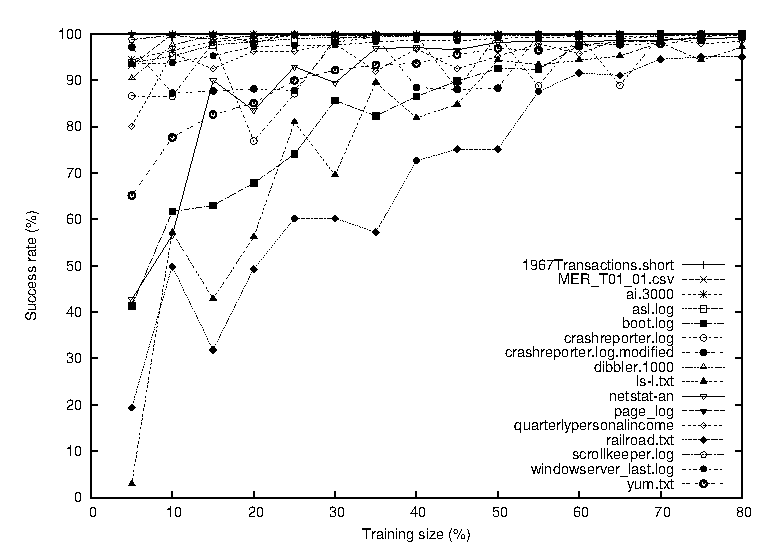
\epsfig{file=successrate.eps, width=\columnwidth}
\caption{Success rates of training sets}
\end{figure}

\begin{figure}
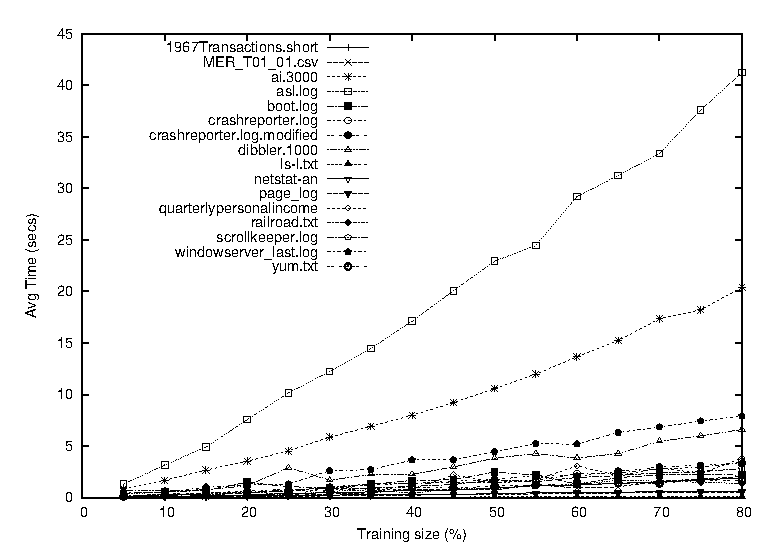
\epsfig{file=traintime.eps, width=\columnwidth}
\caption{Execution times of training sets}
\end{figure}

\begin{table}
\begin{center}
\begin{tabular}{|l|r|l|c|c|} \hline
Title 			& Bytes 	& Ty Comp	& 90\% 		& 95\% \\ \hline \hline
1967Transactions.short	& 70929		& 0.0003	& 5		& 5 			\\ \hline
MER\_T01\_01.csv        & 21731 	& 0.0037	& 5		& 5\\ \hline
ai.3000                 & 293460 	& 0.0004	& 5		& 10\\ \hline
asl.log                 & 279600	& 0.0012	& 5		& 10\\ \hline
boot.log                & 16241		& 0.0213	& 40		& 50\\ \hline
crashreporter.log       & 50152 	& 0.0052	& 5		& 5\\ \hline
crashreporter.log.mod   & 49255		& 0.0053	& 5		& 5\\ \hline
dibbler.1000            & 142607 	& 0.0001	& 5		& 5\\ \hline
ls-l.txt                & 1979		& 0.0461	& 50		& 70\\ \hline
netstat-an              & 14355		& 0.0118	& 20		& 25\\ \hline
page\_log               & 28170		& 0.0032	& 5		& 5\\ \hline
quarterlypersonalincome & 10177		& 0.017		& 10		& 20\\ \hline
railroad.txt            & 6218		& 0.0485	& 60		& 85\\ \hline
scrollkeeper.log        & 66288		& 0.002		& 5		& 5\\ \hline
windowserver\_last.log  & 52394		& 0.0084	& 5		& 10\\ \hline
yum.txt                 & 18221		& 0.0124	& 30		& 40\\ \hline
\end{tabular}
\caption{Min Training size (\%) vs. required accuracy}
\end{center}
\end{table}

\begin{figure}
\begin{center}
\epsfig{file=traintycomp.eps, width=\columnwidth}
\caption{Correlation between structure complexity of 
the data and minimum training size required}
\end{center}
\end{figure}


\section{Conclusion} 
\label{sec:conclusion}

Ad hoc data is pervasive and valuable: in industry, in medicine, and
in scientific research.  Such data tends to have poor documentation,
to contain various kinds of errors, and to be voluminous.  Unlike
well-behaved data in standardized relational or \xml{} formats, such
data has little or no tool support, forcing data analysts and
scientists to waste valuable time writing brittle custom code, even if
all they want to do is convert their data into a well-behaved format.
To improve the situation, various researchers have developed data
description languages such as \pads{}, \datascript{}, and
\packettypes{}.  Such languages allow analysts to write terse,
declarative descriptions of ad hoc data.  A compiler then generates a
parser and customized tools.  Because these languages are tailored to
their domain, they can provide useful services automatically while a
more general purpose tool, such as \lex{}/\yacc{} or \perl{}, cannot.

In the spirit of Landin, we have taken the first steps toward
specifying a semantics for this class of languages by defining the
data description calculus \ddc{}.  This calculus, which is a dependent
type theory with a simple set of orthogonal primitives, is expressive
enough to describe the features of \pads{}, \datascript{}, and
\packettypes{}.  In keeping with the spirit of the data description
languages, our semantics is transformational: instead of simply
recognizing a collection of input strings, we specify how to transform
those strings into canonical in-memory representations annotated with
error information.  Furthermore, we prove that the error information
is meaningful, allowing analysts to rely on the error summaries rather
than having to re-vet the data by-hand.

We have already used the semantics to identify bugs in the
implementation of \padsc{} and to highlight areas where \padsc{}
sacrifices safety for speed.  We have also used the semantics as a guide
for the design of a whole new language, \padsml{}, designed
specifically for functional programmers.  In the future, we hope 
\ddc{} will serve as a solid foundation for the next 700 data 
description languages to come.


\section*{Acknowledgments}
This material is based upon work
 supported by the NSF under grants 0612147 and 0615062, and
a gift from Google. Any opinions, findings, and conclusions or recommendations
expressed in this material are those of the authors and do not
necessarily reflect the views of the NSF or Google.

\bibliographystyle{plain}
%\bibliographystyle{abbrv}

\bibliography{pads}

%\appendix
\section{Language Syntax}
{\allowdisplaybreaks
\noindent
{\bf Syntax of data descriptions and other types}
\label{app:syntax-dd}
\begin{bnf}
\name{Constants} \meta{k} \::= \mcd{true} \| \mcd{false} \| \mcd{()} \| ...
\\
\name{Type Variables} \meta{\alpha}
\\
\name{Type Names} \meta{t}
\\
\name{\Core{} Types} \meta{T} \::= 
  \alpha 
\| {Pbase} 
\| M 
\nlalt \ppair x {T_1} {T_2} 
\| \precord {\nont{ffts}} 
\| \nont{tas}\;t(M) 
\nlalt \pset x T M 
\nlalt \parray T {M_{sep}} {M_{term}} 
\\
\name{\Core{} Datatypes} \meta{D} \::= 
  \mcd{datatype}\; \nont{tps}\; t(x{:}F) = \nont{b} \nlalt
  \mcd{type}\; \nont{tps}\; t(x{:}F) = T
\\
\name{Type Parameters} \meta{tps} \::= \cdot \| \alpha \| (\nont{tvs})
\\
\name{} \meta{tvs} \::= \alpha \| \alpha,\, \nont{tvs}
\\
\name{Type Arguments} \meta{tas} \::= \cdot \| T \| (\nont{ts})
\\
\name{} \meta{ts} \::= T \| T,\, \nont{tss}
\\
\name{} \meta{b} \::= \nont{cs} \| \mcd{case}\; M\; \mcd{of}\; \nont{ccs}
\\
\name{} \meta{cs} \::= c\;\mcd{of}\;T \| c\;\mcd{of}\;T \cvb \nont{cs}
\\
\name{} \meta{ccs} \::= 
  \nont{pat} \Rightarrow c\;\mcd{of}\;T \nlalt
  \nont{pat} \Rightarrow c\;\mcd{of}\;T \cvb \nont{ccs}
\\
\name{\Core{} Field Types} \meta{ffts} \::= \nont{fft} \| \nont{fft};\;\nont{ffts}
\\
\name{\Core{} Field Type} \meta{fft} \::= T \| x = T
\end{bnf}
%\begin{bnf}
\name{Constants} \meta{k} \::= \mcd{true} \| \mcd{false} \| \mcd{()} \| ...
\\
\name{Type Variables} \meta{\alpha}
\\
\name{Type Names} \meta{t}
\\
\name{\Core{} Types} \meta{T} \::= 
  \alpha 
\| {Pbase} 
\| M 
\nlalt \ppair x {T_1} {T_2} 
\| \precord {\nont{ffts}} 
\| \nont{tas}\;t(M) 
\nlalt \pset x T M 
\nlalt \parray T {M_{sep}} {M_{term}} 
\\
\name{\Core{} Datatypes} \meta{D} \::= 
  \mcd{datatype}\; \nont{tps}\; t(x{:}F) = \nont{b} \nlalt
  \mcd{type}\; \nont{tps}\; t(x{:}F) = T
\\
\name{Type Parameters} \meta{tps} \::= \cdot \| \alpha \| (\nont{tvs})
\\
\name{} \meta{tvs} \::= \alpha \| \alpha,\, \nont{tvs}
\\
\name{Type Arguments} \meta{tas} \::= \cdot \| T \| (\nont{ts})
\\
\name{} \meta{ts} \::= T \| T,\, \nont{tss}
\\
\name{} \meta{b} \::= \nont{cs} \| \mcd{case}\; M\; \mcd{of}\; \nont{ccs}
\\
\name{} \meta{cs} \::= c\;\mcd{of}\;T \| c\;\mcd{of}\;T \cvb \nont{cs}
\\
\name{} \meta{ccs} \::= 
  \nont{pat} \Rightarrow c\;\mcd{of}\;T \nlalt
  \nont{pat} \Rightarrow c\;\mcd{of}\;T \cvb \nont{ccs}
\\
\name{\Core{} Field Types} \meta{ffts} \::= \nont{fft} \| \nont{fft};\;\nont{ffts}
\\
\name{\Core{} Field Type} \meta{fft} \::= T \| x = T
\end{bnf}
%%% Local Variables: 
%%% mode: latex
%%% TeX-master: "paper"
%%% End: 


\noindent
{\bf Syntax of terms}
\label{app:syntax-terms}
\begin{bnf}
\name{Types} \meta{F} \::= 
  T           \descr{type of \pvalue{}} 
\nlalt \nont{base} \descr{values of ordinary base types} 
\nlalt \mcd{PD}    \descr{PD type}
\nlalt F * F       \descr{ordinary pairs} 
\nlalt \{\nont{fts}\}     \descr{ordinary records} 
\nlalt F \-> F     \descr{functions}
\nlalt \pstream F  \descr{streams}
\\
\name{Field Types} \meta{fts} \::= x = F \| x=F,\;\nont{fts}
\\
%\end{bnf}
%\begin{bnf}
\name{Parse Descriptors} \meta{pd} \::=   
  G \| B \| N \| S \| U
\\
\name{\Core{} Terms} \meta{N} \::=  
       Pbase[M_1](M_2)                \descr{base type constructor}
\nlalt \langle M \rangle              \descr{unit value (with singleton type M)}
\nlalt (x{=}{M_1} \mathrel{**} {M_2}) \descr{pair}
\nlalt \lcr \nont{fs} \rcr            \descr{record}
\nlalt c[M_1](M_2)                    \descr{data type constructor}
\nlalt \{x = {M_1} \cvb {M_2}\}       \descr{constrained type, with
  $M_2$ the constraint}
\nlalt \mcd{Parray}(M, M_{sep}, M_{term})   \descr{array; first element is stream}
\end{bnf}

\newpage

\begin{bnf}
\name{Terms} \meta{M} \::= 
       x                        \descr{variable}
\nlalt N                        \descr{\core{} terms}
\nlalt k                        \descr{constants}
\nlalt \nont{pd}                      \descr{pd value}
\nlalt (M_1 * M_2)              \descr{ordinary pair}
\nlalt \{\nont{fs}\}        \descr{ordinary record}
\nlalt \tfun {x_1}{x_2}{F_1}{F_2}{M}     \descr{recursive function x1 with arg x2}
\nlalt \mcd{nil}                \descr{empty stream}
\nlalt M_1 \mathrel{::} M_2     \descr{cons}
\nlalt \mcd{case}\;M\;\mcd{of}\;\nont{ms} \descr{deconstructors}
\nlalt M_1\;(M_2)               \descr{function application}
\nlalt \mcd{op}\;M                     \descr{additional uninteresting operations}
\nlalt \mcd{let}\;x = M_1\;\mcd{in}\;M_2           \descr{computation in host language}
\nlalt \mcd{cast}\;(M : T)             \descr{type annot/dependent cast?}
\\
\name{Fields} \meta{fs} \::= x = M \| x = M; \nont{fs}
\\
\name{Matches}\meta{ms} \::= 
  \nont{pat} \Rightarrow M \| \nont{pat} \Rightarrow M \cvb \nont{ms}
\end{bnf}
%{\small
\begin{verbatim}
M ::=  x                        // variable
     | Pbase[M1](M2)            // base type constructor; M1 is
                                   an argument to the type; M2 computes the rep)
     | c(M)                     // data type constructor with parameter M
     | (x:M1 ** M2)             // pair
     | {fields}                 // record
     | {x = M1 | M2}            // set-type; M2 is the predicate
     | Parray(M, Msep, Mterm)   // array; first element is stream
     | k                        // constants
     | let x = M in M           // computation in host language
     | <M>                      // unit value given singleton type M
     | (M1 * M2)                // ordinary pair
     | nil                      // empty list
     | M1 :: M2                 // cons
     | case M of MS             // deconstructors
     | fun x1(x2:F1):F2 = M     // recursive function x1 with arg x2
     | M1 (M2)                  // function application
     | cast (M : T)             // type annot/dependent cast?
     | op M                     // additional uninteresting operations
     
fields ::= x = M | x = M; fields

pd ::=   G    // good
     |   B    // bad
     |   N    // nested error
     |   S    // semantic error
     |   U    // unknown
\end{verbatim}
}

  
\newpage

\noindent
{\bf Syntax of patterns}
\label{app:syntax-pat}
\begin{bnf}
% \name{Parse Descriptors} \meta{pd} \::=   
%          G    \descr{good}
% \nlalt   B    \descr{bad}
% \nlalt   N    \descr{nested error}
% \nlalt   S    \descr{semantic error}
% \nlalt   U    \descr{unknown}
\name{\Core{} Patterns} \meta{fpat} \::=
x \| \nont{Pbase}(\nont{pat})
\nlalt \langle \nont{pat} \rangle             \descr{singleton}
\nlalt (\nont{fpat} \mathrel{**} \nont{fpat})   \descr{\core{} pair}
\nlalt \lcr \nont{ffps} \rcr                  \descr{\core{} record}
\nlalt c(\nont{fpat})                          \descr{constructor}
\nlalt \{\nont{fpat} \cvb \nont{cpat}\}        \descr{type constaint}
\nlalt \mcd{Parray}(\nont{pat}, x_{sep}, x_{term}) \descr{array with stream, sep and term.}
\nlalt \nont{fpat}\langle\langle\nont{pdpat}\rangle\rangle
\\
\name{Patterns}\meta{pat} \::= 
       \nont{fpat} \descr{\core{} pattern}
\nlalt k \| \nont{pdpat}                      \descr{constants and parse descriptors}
\nlalt (\nont{pat} * \nont{pat})              \descr{normal pair}
\nlalt \{\nont{fps}\}                        \descr{record}
\nlalt \mcd{nil} \| \nont{pat}_1 \mathrel{::} \nont{pat}_2 \descr{stream}
\\
\name{\Core{} Field Pattern} \meta{ffps} \::= x = \nont{fpat} \| x = \nont{fpat};\;\nont{ffps}
\\
\name{Constraint Pattern} \meta{cpat} \::= x \| \mcd{true} \| \mcd{false}
\\
\name{PD Pattern} \meta{pdpat}\::= x \| \nont{pd}
\\
\name{Field Pattern} \meta{fps} \::= x = \nont{pat} \| x = \nont{pat};\;\nont{fps}
\end{bnf}
%{\small
\begin{bnf}
% \name{Parse Descriptors} \meta{pd} \::=   
%          G    \descr{good}
% \nlalt   B    \descr{bad}
% \nlalt   N    \descr{nested error}
% \nlalt   S    \descr{semantic error}
% \nlalt   U    \descr{unknown}
\name{\Core{} Patterns} \meta{fpat} \::=
x \| \nont{Pbase}(\nont{pat})
\nlalt \langle \nont{pat} \rangle             \descr{singleton}
\nlalt (\nont{fpat} \mathrel{**} \nont{fpat})   \descr{\core{} pair}
\nlalt \lcr \nont{ffps} \rcr                  \descr{\core{} record}
\nlalt c(\nont{fpat})                          \descr{constructor}
\nlalt \{\nont{fpat} \cvb \nont{cpat}\}        \descr{type constaint}
\nlalt \mcd{Parray}(\nont{pat}, x_{sep}, x_{term}) \descr{array with stream, sep and term.}
\nlalt \nont{fpat}\langle\langle\nont{pdpat}\rangle\rangle
\\
\name{Patterns}\meta{pat} \::= 
       \nont{fpat} \descr{\core{} pattern}
\nlalt k \| \nont{pdpat}                      \descr{constants and parse descriptors}
\nlalt (\nont{pat} * \nont{pat})              \descr{normal pair}
\nlalt \{\nont{fps}\}                        \descr{record}
\nlalt \mcd{nil} \| \nont{pat}_1 \mathrel{::} \nont{pat}_2 \descr{stream}
\\
\name{\Core{} Field Pattern} \meta{ffps} \::= x = \nont{fpat} \| x = \nont{fpat};\;\nont{ffps}
\\
\name{Constraint Pattern} \meta{cpat} \::= x \| \mcd{true} \| \mcd{false}
\\
\name{PD Pattern} \meta{pdpat}\::= x \| \nont{pd}
\\
\name{Field Pattern} \meta{fps} \::= x = \nont{pat} \| x = \nont{pat};\;\nont{fps}
\end{bnf}
}

%%% Local Variables: 
%%% mode: latex
%%% TeX-master: "paper"
%%% End: 


\noindent
{\bf Syntax of programs}
\label{app:syntax-prog}
\begin{bnf}
\name{Program} \meta{prog} \::= 
  M              
 \nlalt D\; \nont{prog}          \descr{type declaration}
 \nlalt \mcd{val}\;x = M\;\mcd{prog} \descr{value declaration}
\end{bnf}
%{\small
\begin{verbatim}
prog ::= M              
       | D prog          // type declaration
       | val x = M prog  // value declaration
\end{verbatim}
}

}
%%% Local Variables: 
%%% mode: latex
%%% TeX-master: "paper"
%%% End: 


\end{document}

%%% Local Variables:
%%% mode: outline-minor
%%% End:

